\documentclass[titlepage,a4paper]{article}
\usepackage{a4wide}
\usepackage[T1]{fontenc}
\usepackage{lipsum}
\usepackage{enumitem,amssymb}
\newlist{todolist}{itemize}{2}
\setlist[todolist]{label=$\square$}
\usepackage{pifont}
\usepackage{xcolor}
\usepackage[normalem]{ulem}
\usepackage{listings}
\usepackage{color}
\usepackage{pdfpages}
\usepackage{multirow}
\usepackage{plantuml}
\usepackage{fancyhdr}
\usepackage{float}
\usepackage[spanish,es-tabla]{babel}

% Quote box
% for adjustwidth environment
\usepackage[strict]{changepage}

% for formal definitions
\usepackage{framed}

% Add the titlesec package for optional formatting (if needed)
\usepackage{titlesec}

\newcounter{subsubsubsection}[subsubsection]
\renewcommand\thesubsubsubsection{\thesubsubsection.\arabic{subsubsubsection}}
\renewcommand\theparagraph{\thesubsubsubsection.\arabic{paragraph}} % optional; useful if paragraphs are to be numbered

\titleformat{\subsubsubsection}
  {\normalfont\normalsize\bfseries}{\thesubsubsubsection}{1em}{}
\titlespacing*{\subsubsubsection}
{0pt}{3.25ex plus 1ex minus .2ex}{1.5ex plus .2ex}

\makeatletter
\renewcommand\paragraph{\@startsection{paragraph}{5}{\z@}%
  {3.25ex \@plus1ex \@minus.2ex}%
  {-1em}%
  {\normalfont\normalsize\bfseries}}
\renewcommand\subparagraph{\@startsection{subparagraph}{6}{\parindent}%
  {3.25ex \@plus1ex \@minus .2ex}%
  {-1em}%
  {\normalfont\normalsize\bfseries}}
\def\toclevel@subsubsubsection{4}
\def\toclevel@paragraph{5}
\def\toclevel@paragraph{6}
\def\l@subsubsubsection{\@dottedtocline{4}{7em}{4em}}
\def\l@paragraph{\@dottedtocline{5}{10em}{5em}}
\def\l@subparagraph{\@dottedtocline{6}{14em}{6em}}
\makeatother

\setcounter{secnumdepth}{5}
\setcounter{tocdepth}{4}


% environment derived from framed.sty: see leftbar environment definition
\definecolor{formalshade}{rgb}{0.95,0.95,1}

\newenvironment{formal}{%
  \def\FrameCommand{%
    \hspace{1pt}%
    {\color{blue}\vrule width 2pt}%
    {\color{formalshade}\vrule width 4pt}%
    \colorbox{formalshade}%
  }%
  \MakeFramed{\advance\hsize-\width\FrameRestore}%
  \noindent\hspace{-4.55pt}% disable indenting first paragraph
  \begin{adjustwidth}{}{7pt}\itshape%
  \vspace{2pt}\vspace{2pt}%
}
{%
  \vspace{2pt}\end{adjustwidth}\endMakeFramed%
}

\definecolor{dkgreen}{rgb}{0,0.6,0}
\definecolor{gray}{rgb}{0.5,0.5,0.5}
\definecolor{mauve}{rgb}{0.58,0,0.82}

\lstset{frame=tb,
  language=Java,
  aboveskip=3mm,
  belowskip=3mm,
  showstringspaces=false,
  columns=flexible,
  basicstyle={\small\ttfamily},
  numbers=none,
  numberstyle=\tiny\color{gray},
  keywordstyle=\color{blue},
  commentstyle=\color{dkgreen},
  stringstyle=\color{mauve},
  breaklines=true,
  breakatwhitespace=true,
  tabsize=3,
  literate=
  {á}{{\'a}}1 {é}{{\'e}}1 {í}{{\'i}}1 {ó}{{\'o}}1 {ú}{{\'u}}1
  {Á}{{\'A}}1 {É}{{\'E}}1 {Í}{{\'I}}1 {Ó}{{\'O}}1 {Ú}{{\'U}}1
  {à}{{\`a}}1 {è}{{\`e}}1 {ì}{{\`i}}1 {ò}{{\`o}}1 {ù}{{\`u}}1
  {À}{{\`A}}1 {È}{{\'E}}1 {Ì}{{\`I}}1 {Ò}{{\`O}}1 {Ù}{{\`U}}1
  {ä}{{\"a}}1 {ë}{{\"e}}1 {ï}{{\"i}}1 {ö}{{\"o}}1 {ü}{{\"u}}1
  {Ä}{{\"A}}1 {Ë}{{\"E}}1 {Ï}{{\"I}}1 {Ö}{{\"O}}1 {Ü}{{\"U}}1
  {â}{{\^a}}1 {ê}{{\^e}}1 {î}{{\^i}}1 {ô}{{\^o}}1 {û}{{\^u}}1
  {Â}{{\^A}}1 {Ê}{{\^E}}1 {Î}{{\^I}}1 {Ô}{{\^O}}1 {Û}{{\^U}}1
  {ã}{{\~a}}1 {ẽ}{{\~e}}1 {ĩ}{{\~i}}1 {õ}{{\~o}}1 {ũ}{{\~u}}1
  {Ã}{{\~A}}1 {Ẽ}{{\~E}}1 {Ĩ}{{\~I}}1 {Õ}{{\~O}}1 {Ũ}{{\~U}}1
  {œ}{{\oe}}1 {Œ}{{\OE}}1 {æ}{{\ae}}1 {Æ}{{\AE}}1 {ß}{{\ss}}1
  {ű}{{\H{u}}}1 {Ű}{{\H{U}}}1 {ő}{{\H{o}}}1 {Ő}{{\H{O}}}1
  {ç}{{\c c}}1 {Ç}{{\c C}}1 {ø}{{\o}}1 {å}{{\r a}}1 {Å}{{\r A}}1
  {€}{{\euro}}1 {£}{{\pounds}}1 {«}{{\guillemotleft}}1
  {»}{{\guillemotright}}1 {ñ}{{\~n}}1 {Ñ}{{\~N}}1 {¿}{{?`}}1 {¡}{{!`}}1
}

\pagestyle{fancy} % Encabezado y pie de página
\fancyhf{}
\fancyhead[L]{Trabajo Práctico Final | Jazz Jackrabbit 2 | Grupo 5\\Manual de Usuario}
\fancyhead[R]{Taller de Programación I - FIUBA}
\renewcommand{\headrulewidth}{0.4pt}
\fancyfoot[C]{\thepage}
\renewcommand{\footrulewidth}{0.4pt}

\fancypagestyle{firstPage}{%
  \fancyfoot[C]{\thepage}
  \renewcommand{\footrulewidth}{0.4pt}
}

\begin{document}

\begin{titlepage} % Carátula
	\hfill
\includegraphics[width=6cm]{logofiuba.jpg}
    \centering
    \vfill
    \Huge \textbf{Trabajo Práctico Final\\Jazz Jackrabbit 2}
    \vskip2cm
    \Large [75.42] Taller de Programación I\\
    Primer Cuatrimestre de 2024
    \vfill
    \begin{tabular}{ | l | l | l | } % Datos del alumno
      \hline
      \textbf{Estudiante} & \textbf{Padrón} & \textbf{Email} \\ \hline
      Buono, Fernando & 103523 & fbuono@fi.uba.ar \\ \hline
      Duca, Francisco & 106308 & fduca@fi.uba.ar \\ \hline
      Oshiro, Lucas & 107024 & loshiro@fi.uba.ar \\ \hline
      Shiao, Tomás Jorge & 106099 & tshiao@fi.uba.ar \\ \hline
  	\end{tabular}
    \vfill
    \vfill
\end{titlepage}

\clearpage\pagestyle{empty}
\tableofcontents % Índice general
\newpage
\setcounter{page}{1}
\pagestyle{fancy}
\setcounter{secnumdepth}{5}
\setcounter{tocdepth}{5}
\section{Sistema Operativo}
El presente proyecto fue probado en los sistemas operativos Ubuntu 22.04 LTS y MX Linux. No se garantiza su correcto funcionamiento en otros sistemas operativos.

\section{Dependencias}
Se adjunta en el repositorio un archivo \texttt{installer.sh} que, ejecutándolo, instalará las dependencias necesarias para compilar y ejecutar el proyecto. Para ejecutarlo, se debe correr el siguiente comando en la terminal:

\begin{lstlisting}[language=sh,caption=Ejecución del Instalador, captionpos=b]
  $ chmod +x installer.sh # Para darle permisos de ejecución
  $ ./installer.sh
\end{lstlisting}

Si se prefiere instalar las dependencias manualmente, se deben instalar las siguientes bibliotecas:

\begin{enumerate}
  \item SDL2
  \begin{enumerate}
    \item SDL2pp
    \item SDL2\_image
    \item SDL2\_mixer
    \item SDL2\_ttf
  \end{enumerate}
  \item QT5
  \item CMake
  \item GTest
  \item libfmt
  \item yaml-cpp
\end{enumerate}

Se asume que el usuario que instala manualmente las dependencias conoce cómo instalarlas en su sistema operativo y cómo configurarlo, si es que es necesario. En caso que no, se puede consultar el script provisto.

\section{Configuración}
La única configuración necesaria es la instalación de la tipografía, que se provee en el repositorio en \texttt{assets/Miscellaneous/Jazz-Jackrabbit-2.ttf}. Para instalarla, se debe ejecutar:

\begin{lstlisting}[language=sh,caption=Instalación de la Tipografía, captionpos=b]
  $ sudo cp assets/Miscellaneous/Jazz-Jackrabbit-2.ttf /usr/share/fonts/
  $ fc-cache -f -v
\end{lstlisting}

\section{Utilizando Vagrant}
El proyecto también provee un archivo \texttt{Vagrantfile} que permite crear una máquina virtual con todas las dependencias necesarias para compilar y ejecutar el proyecto. Para ello, se debe tener instalado Vagrant y VirtualBox.

Para crear la máquina virtual y correr el proyecto, en la carpeta donde se bajó el código del repositorio, se debe ejecutar:

\begin{lstlisting}[language=sh,caption=Creación de la Máquina Virtual, captionpos=b]
  $ vagrant up  --provision
  $ vagrant ssh
  $ cd /home/vagrant/jazz_jackrabbit_2/build
  $ ./jazzserver <port> # Para correr el servidor, reemplazar <port> por un puerto a elección
  $ ./jazzclient <ip> <port> # Para correr el cliente, reemplazar <ip> por la IP del servidor (localhost) y <port> por el puerto
  $ ./leveleditor # Para ejecutar el editor de niveles
\end{lstlisting}

El archivo \texttt{Vagrantfile} se encarga de instalar las dependencias necesarias y compilar el proyecto. Para correr el servidor y el cliente, se debe ejecutar el servidor primero y luego el cliente.

Para salir de Vagrant, una vez finalizada la ejecución:

\begin{lstlisting}[language=sh,caption=Salir de Vagrant, captionpos=b]
  $ exit
  $ vagrant halt
  $ vagrant destroy # Si se desea borrar la máquina virtual
\end{lstlisting}

\section{Compilación y Ejecución}
Para compilar el proyecto, se debe ejecutar los siguientes comandos en la terminal:

\begin{lstlisting}[language=sh,caption=Compilación del Proyecto, captionpos=b]
  $ sudo rm -rf build # Si es que existe una carpeta build previa
  $ mkdir -p build
  $ cd build
  $ cmake ..
  $ make -j$(nproc) # Alternativamente, make -j4
\end{lstlisting}

Una vez compilado, para ejecutar el servidor se debe correr:

\begin{lstlisting}[language=sh,caption=Ejecución del Servidor, captionpos=b]
  $ ./jazzserver <port> # Reemplazar <port> por un puerto a elección
\end{lstlisting}

Para ejecutar el cliente, se debe ejecutar:

\begin{lstlisting}[language=sh,caption=Ejecución del Cliente, captionpos=b]
  $ ./jazzclient <ip> <port> # Reemplazar <ip> por la IP del servidor (localhost) y <port> por el puerto
\end{lstlisting}

Por último, para el editor de niveles:

\begin{lstlisting}[language=sh,caption=Ejecución del Editor de Niveles, captionpos=b]
  $ ./leveleditor
\end{lstlisting}

\section{Lobby}
El Lobby es donde el usuario selecciona qué quiere hacer: crear o unirse a una partida. Consiste de las siguientes pantallas:

\begin{figure}[H]
  \centering
  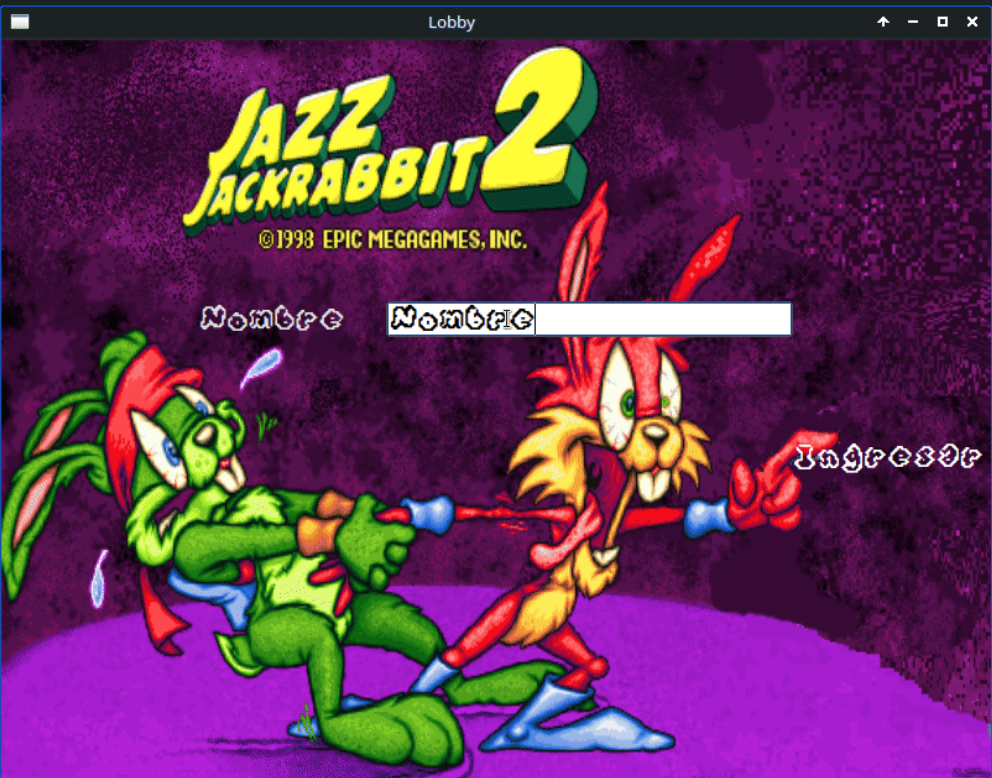
\includegraphics[width=0.8\textwidth]{images/Lobby/Welcome.png}
  \caption{Pantalla de Bienvenida}
  \label{fig:welcome}
\end{figure}

En esta primera pantalla, solamente se pide que el usuario ingrese su nombre. 

\begin{figure}[H]
  \centering
  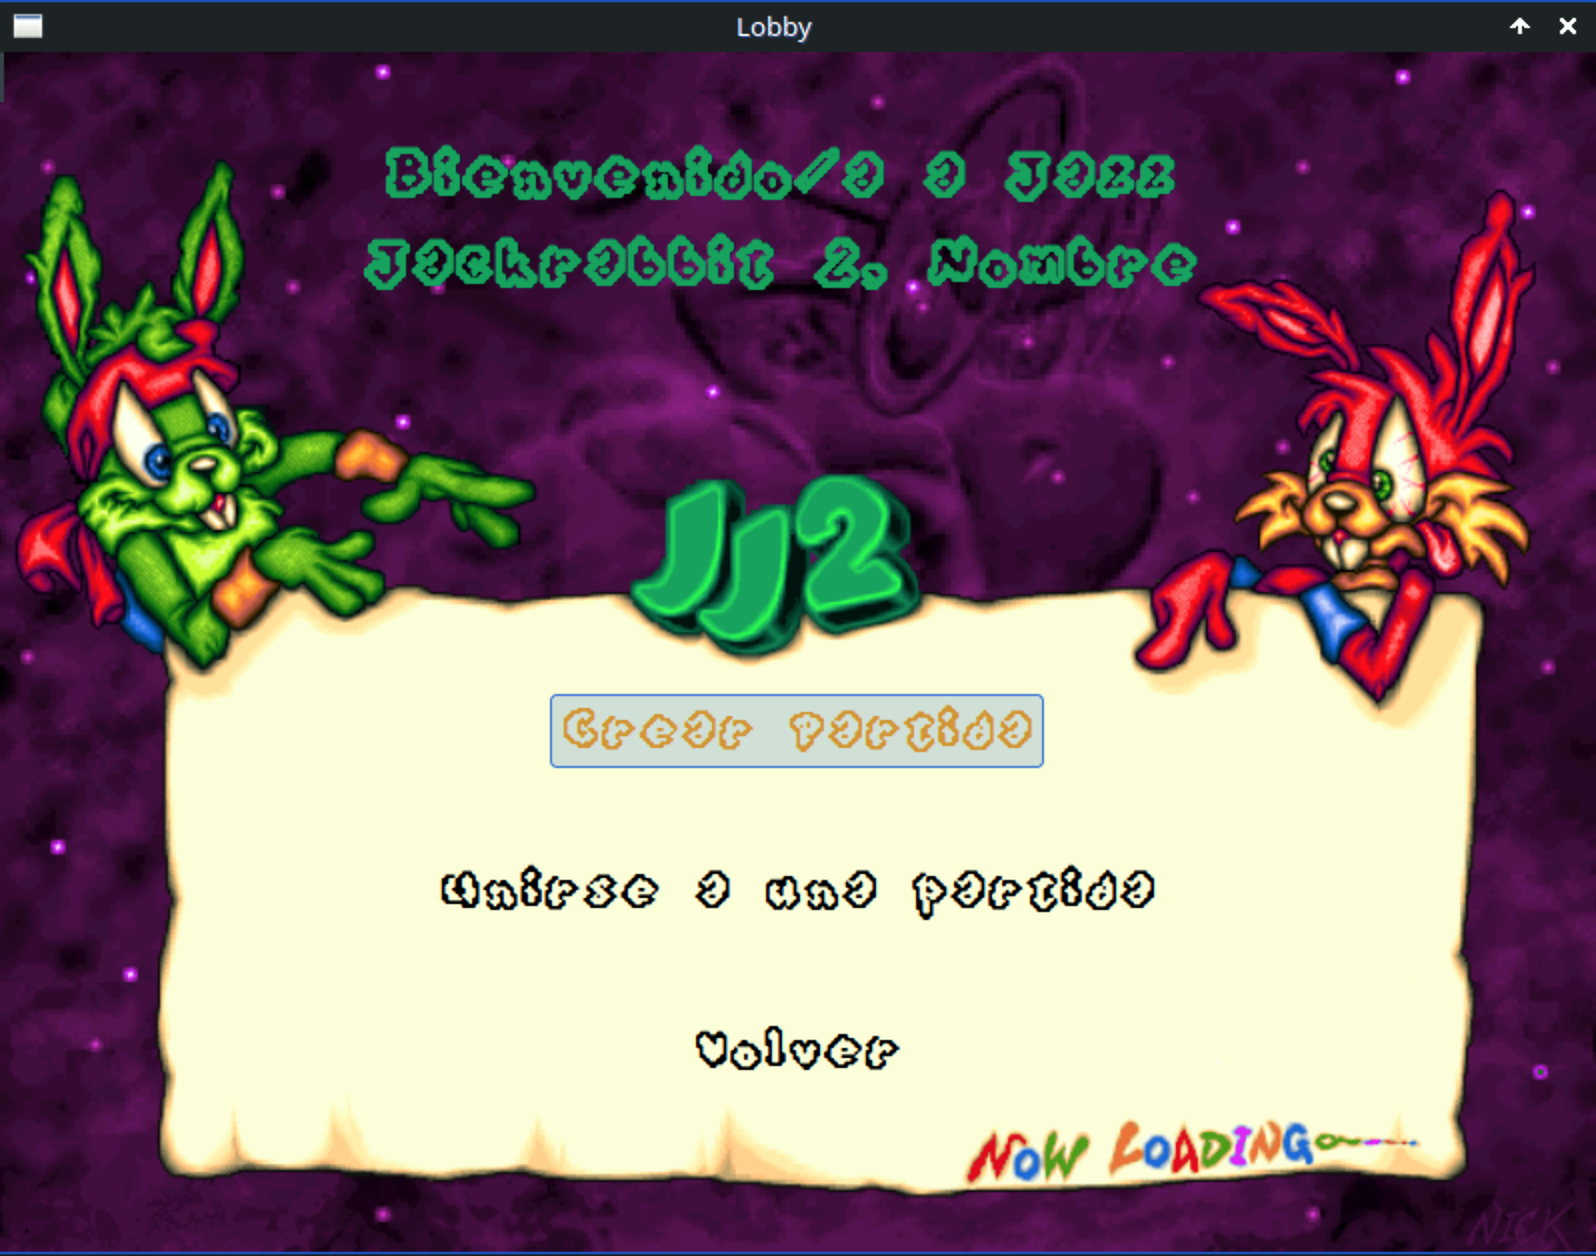
\includegraphics[width=0.8\textwidth]{images/Lobby/Lobby.png}
  \caption{Menú Principal}
  \label{fig:lobby}
\end{figure}

Luego de ingresar su nombre, se llega al menú principal. Es aquí donde se elige si se quiere crear una partida o unirse a una.

Si se selecciona la creación de uina partida, se procede a la selección del escenario de juego:

\begin{figure}[H]
  \centering
  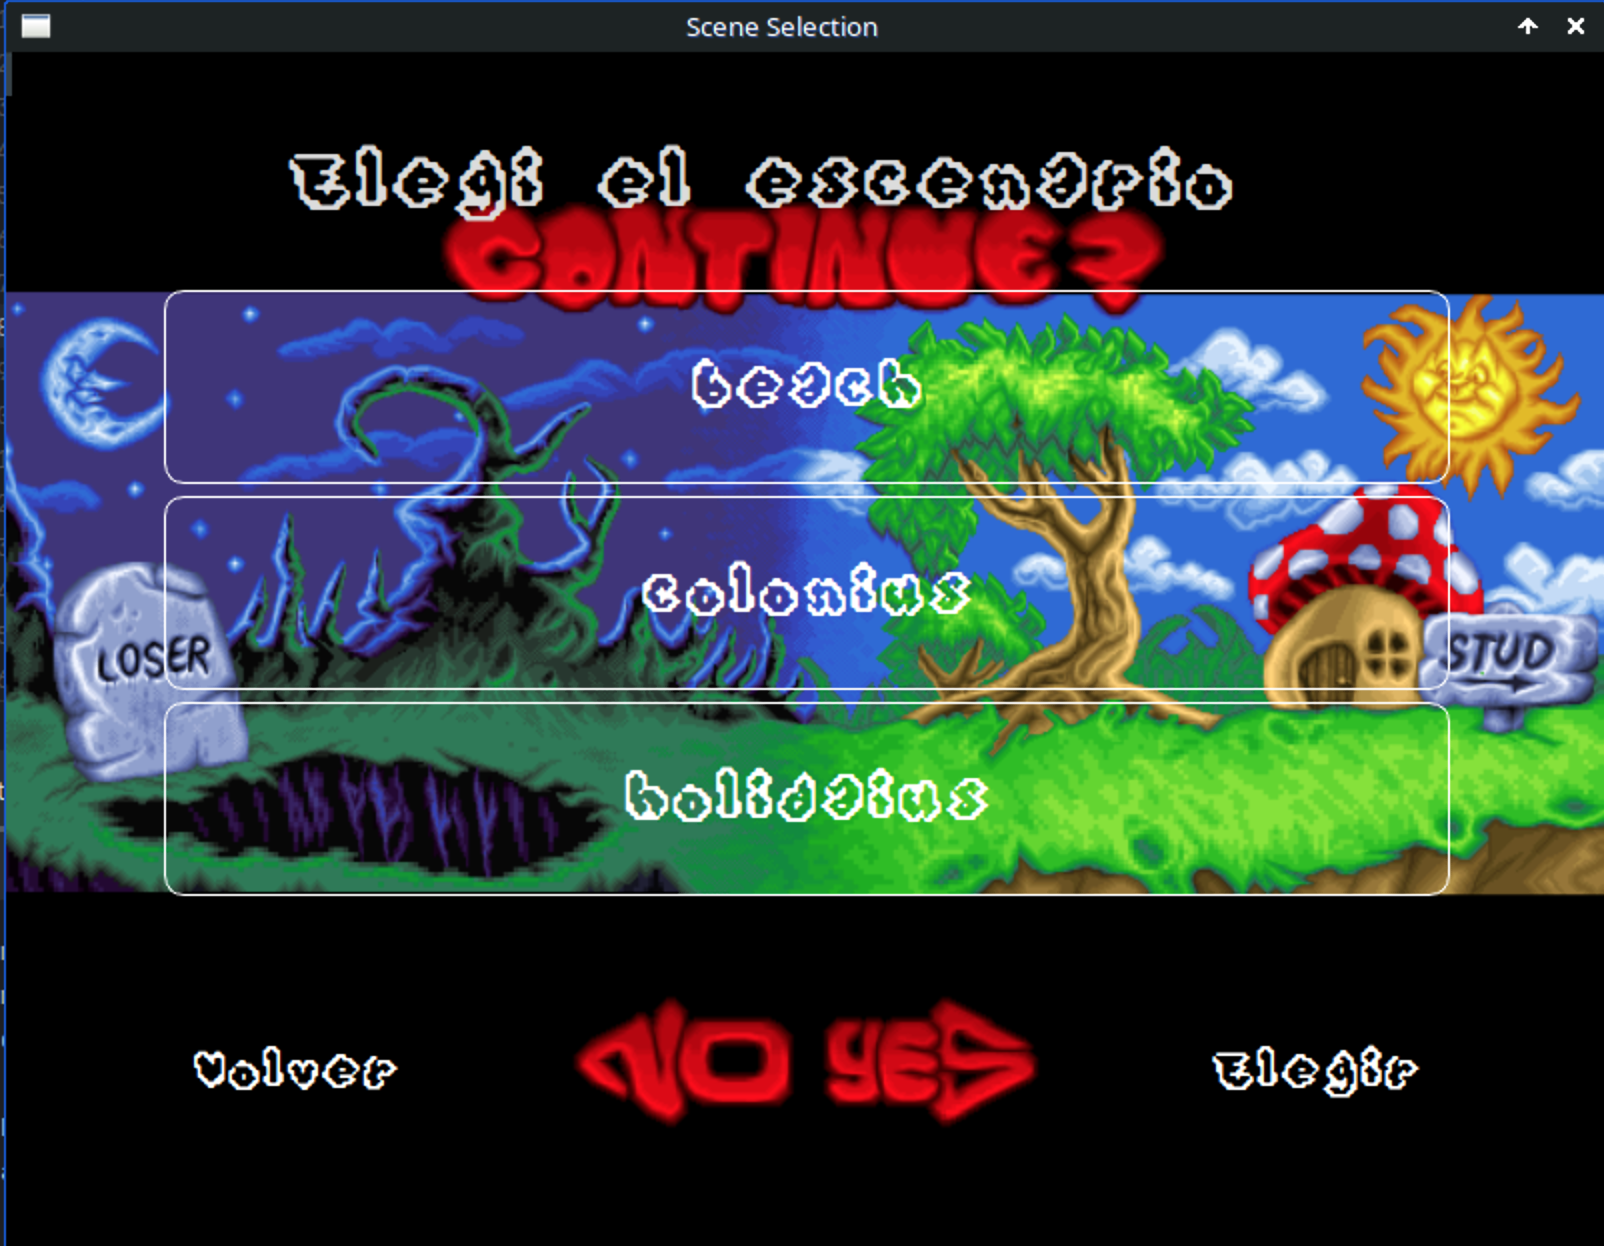
\includegraphics[width=0.8\textwidth]{images/Lobby/SceneSelection.png}
  \caption{Selección de Escenario}
  \label{fig:scene}
\end{figure}

Luego, la configuración de la partida a crear:

\begin{figure}[H]
  \centering
  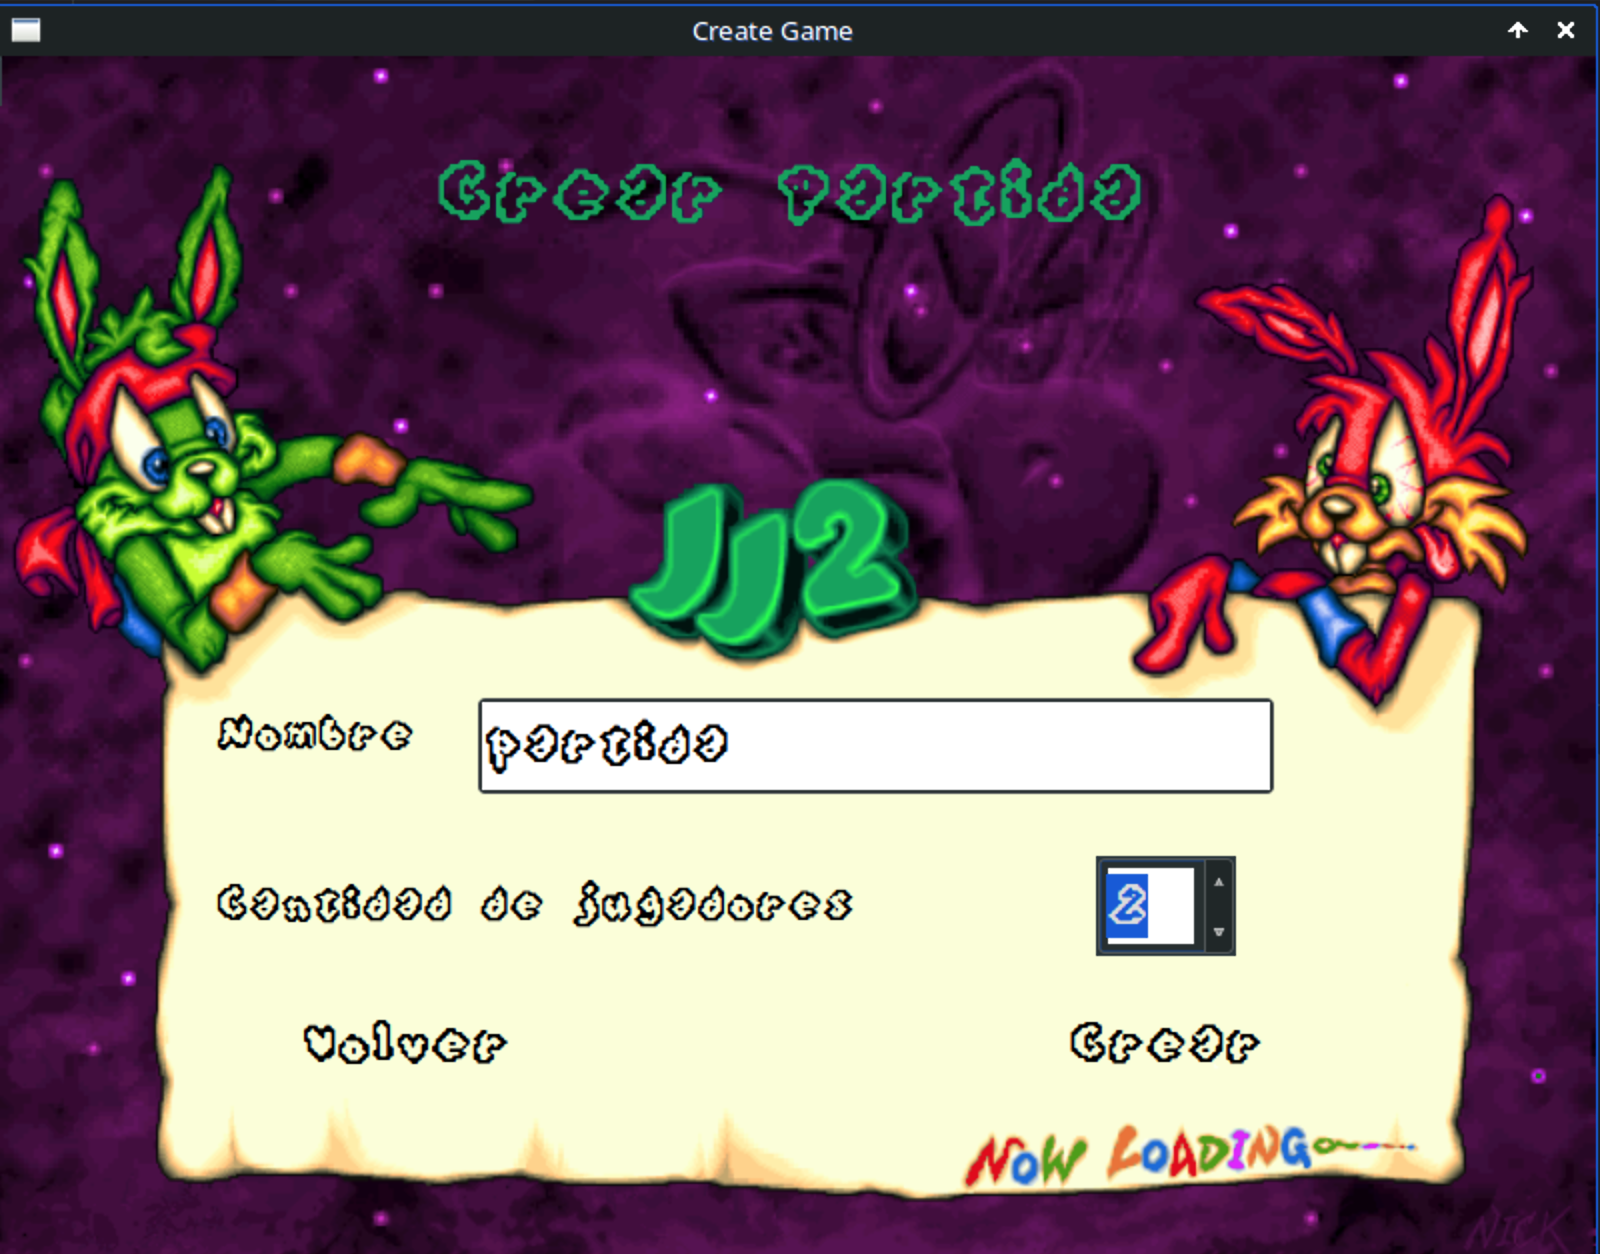
\includegraphics[width=0.8\textwidth]{images/Lobby/CreateGame.png}
  \caption{Configuración de la Partida}
  \label{fig:create}
\end{figure}

Aquí se nombra una partida y se decide la cantidad de jugadores que tendrá, donde se limita a un máximo de 3 personas.

El siguiente paso es la selección del personaje con el que se desea jugar:

\begin{figure}[H]
  \centering
  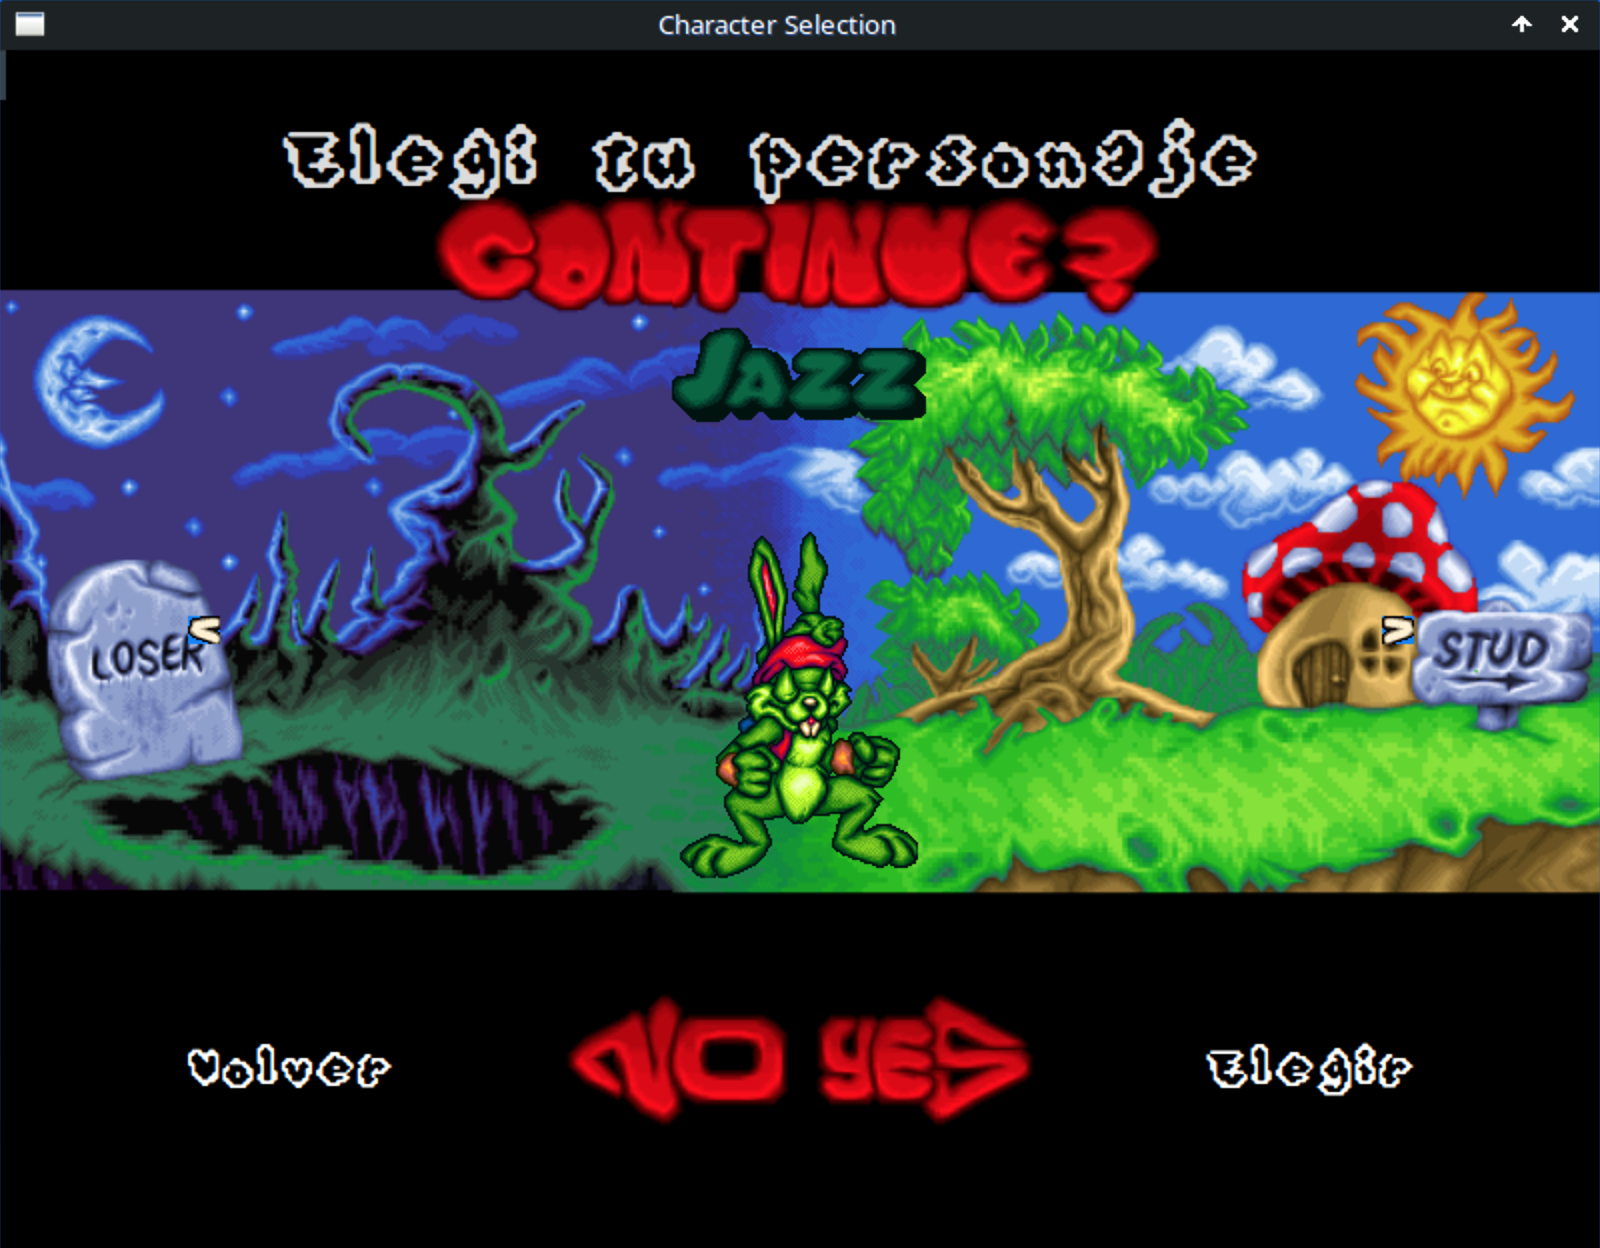
\includegraphics[width=0.8\textwidth]{images/Lobby/CharacterSelection.png}
  \caption{Selección de Personaje}
  \label{fig:character}
\end{figure}

En el caso de que la partida sea de múltiples jugadores, se entrará a la sala de espera:

\begin{figure}[H]
  \centering
  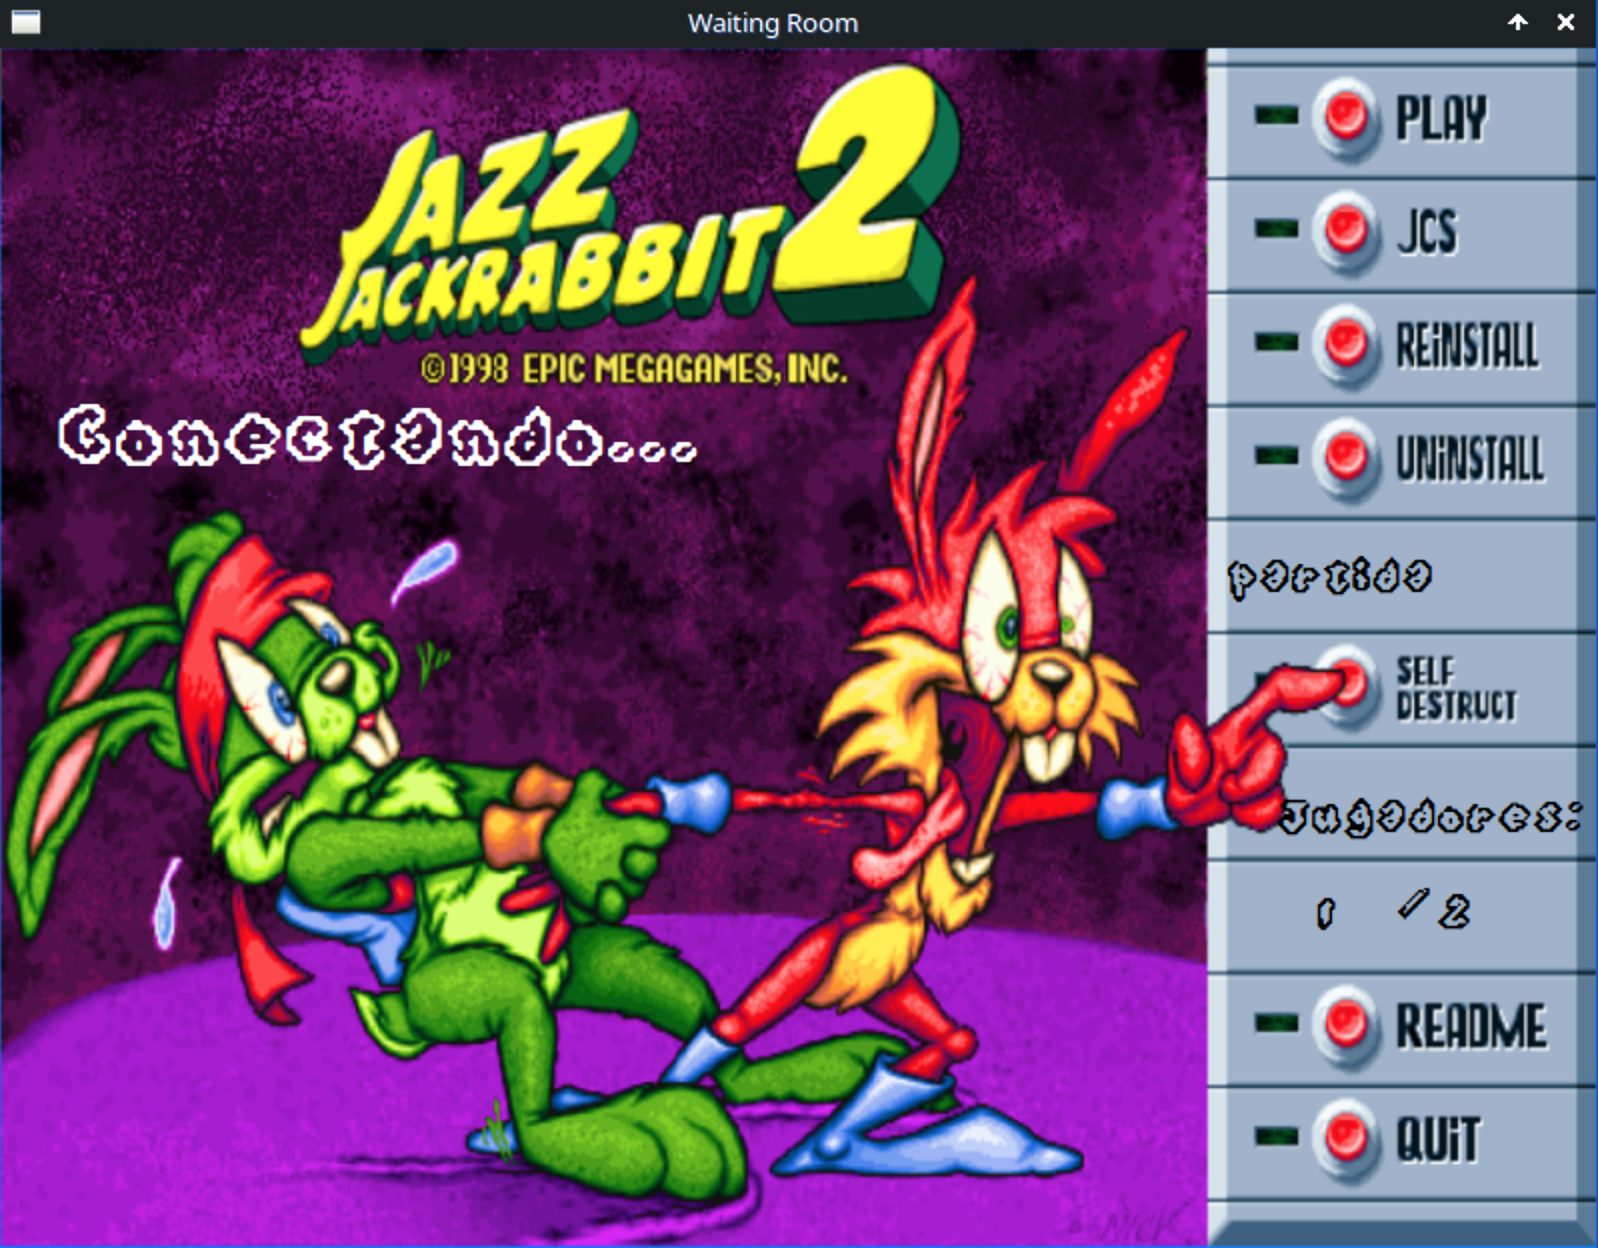
\includegraphics[width=0.8\textwidth]{images/Lobby/WaitingRoom.png}
  \caption{Sala de Espera}
  \label{fig:waiting-room}
\end{figure}

En el caso de que se seleccione para unirse a una partida, se procederá primero a la selección del personaje, como se muestra en la Figura \ref{fig:character}.

Luego de eso, se muestra la pantalla de selección de partidas, donde si no hay partidas se muestra:

\begin{figure}[H]
  \centering
  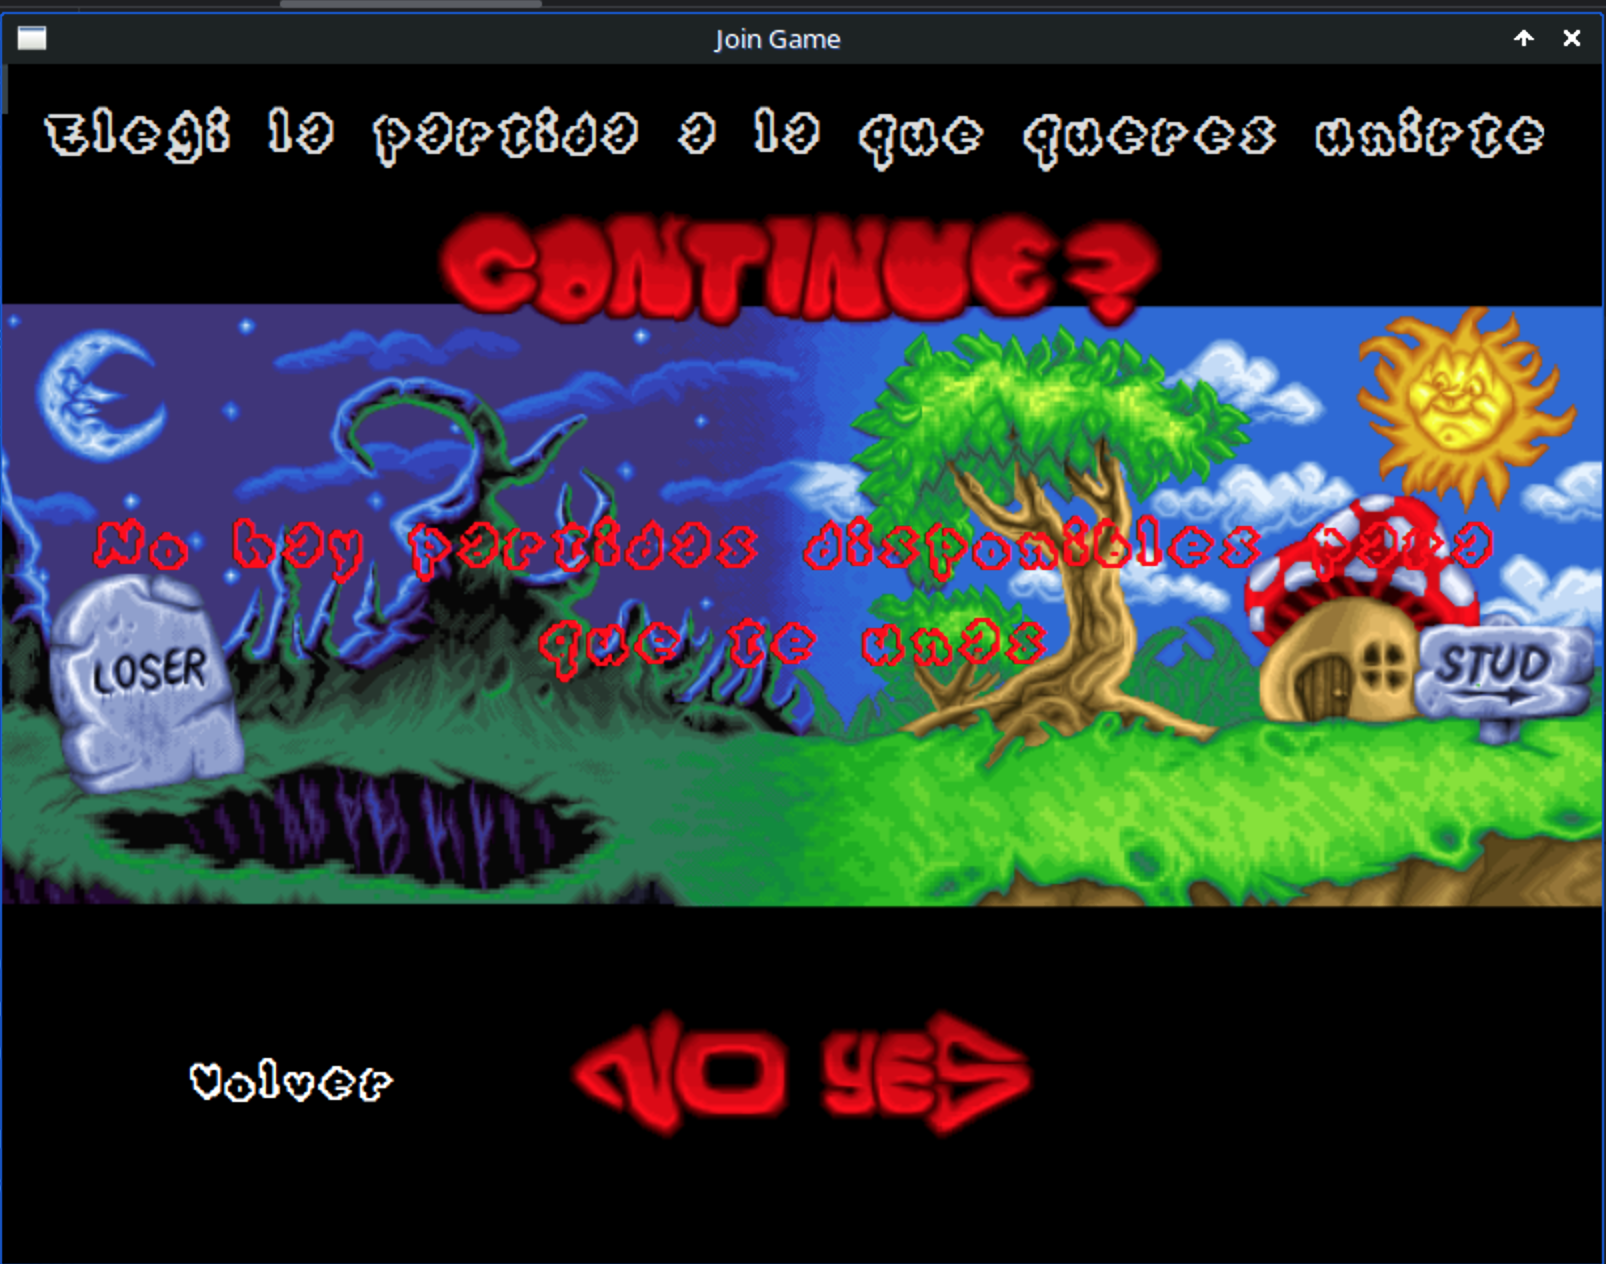
\includegraphics[width=0.8\textwidth]{images/Lobby/GamesListNoGames.png}
  \caption{No hay Partidas}
  \label{fig:no-games}
\end{figure}

En el caso que sí:

\begin{figure}[H]
  \centering
  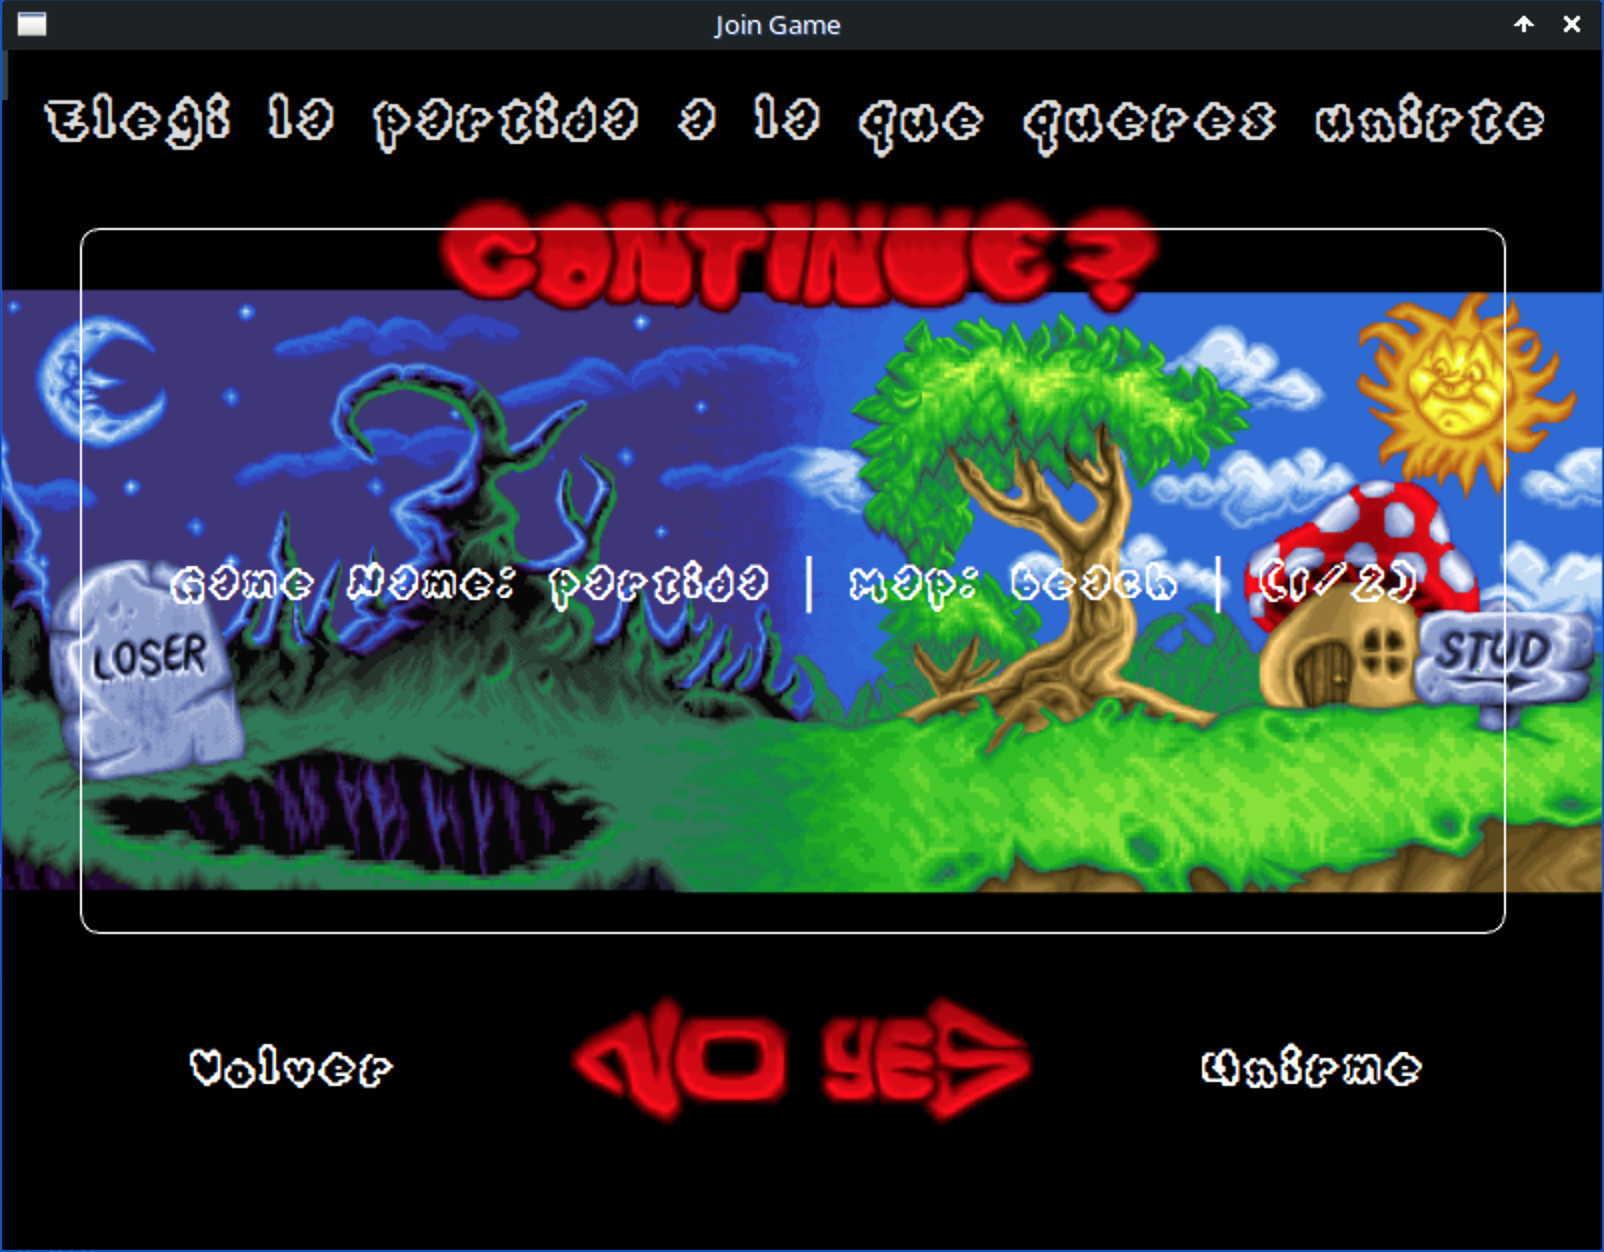
\includegraphics[width=0.8\textwidth]{images/Lobby/GamesList.png}
  \caption{Lista de Partidas}
  \label{fig:games-list}
\end{figure}

En caso que aún falten jugadores para que la partida comience, se mostrará la sala de espera, como se muestra en la Figura \ref{fig:waiting-room}. En caso contrario, el juego arranca para todos los jugadores.


\section{Juego} 
El juego consiste en un escenario con plataformas y obstáculos, donde los jugadores deben recolectar diamantes y disparar a los otros jugadores para obtener puntos. El juego termina cuando se acaba el tiempo.

\begin{enumerate}
  \item Movimientos: estos se realizan con las teclas \texttt{D} hacia la derecha y \texttt{A} hacia la izquierda.
  \item Salto: se realiza con la tecla \texttt{espacio}.
  \item Disparo: se realiza con la tecla \texttt{M}.
  \item Correr más rápido: se realiza con la tecla \texttt{SHIFT} de la izquierda.
  \item Cambiar de arma: se realiza con la tecla \texttt{G}.
  \item Ataque especial: se realiza con la tecla \texttt{V}.
\end{enumerate}

\begin{figure}[H]
  \centering
  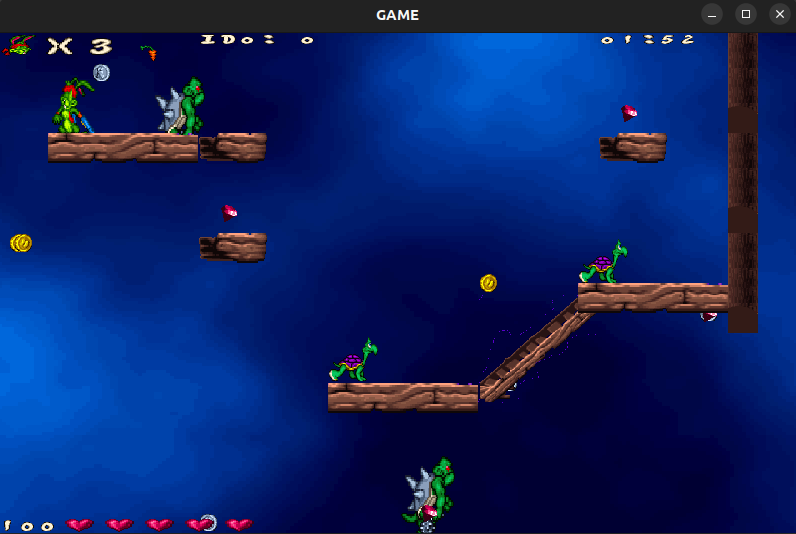
\includegraphics[width=0.8\textwidth]{images/gameScreen.png}
  \caption{Captura del Juego}
  \label{fig:game}
\end{figure}

\section{Editor de Niveles}
El editor de niveles consiste en una sola pantalla:

\begin{figure}[H]
  \centering
  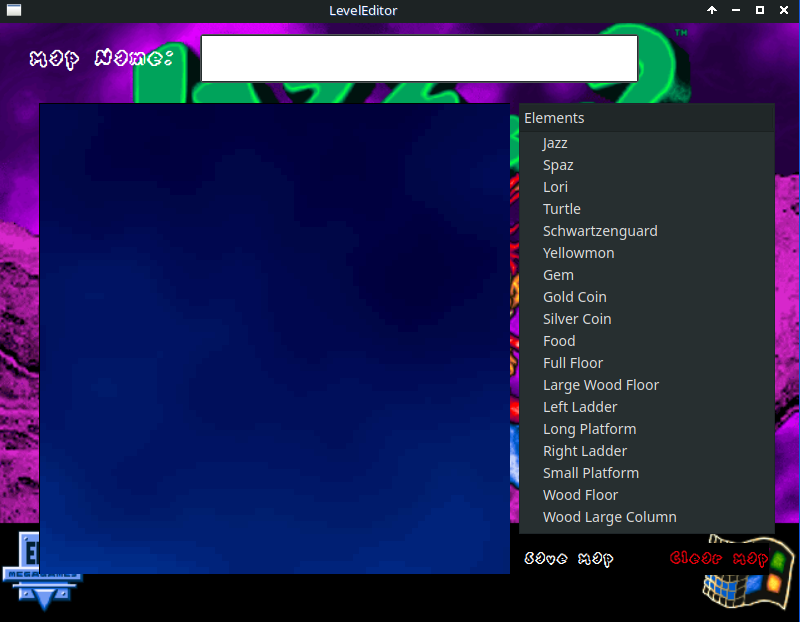
\includegraphics[width=0.8\textwidth]{images/LevelEditor/LevelEditor.png}
  \caption{Editor de Niveles}
  \label{fig:level-editor}
\end{figure}

El mapa necesita un nombre, que tenga elementos y que no exista un mapa con el mismo nombre creado previamente. Se pueden agregar y quitar elementos del mapa, como se muestra en la Figura \ref{fig:level-editor}.

En caso que no se cumpla alguna de las condiciones previas:

Si el mapa no tiene nombre:

\begin{figure}[H]
  \centering
  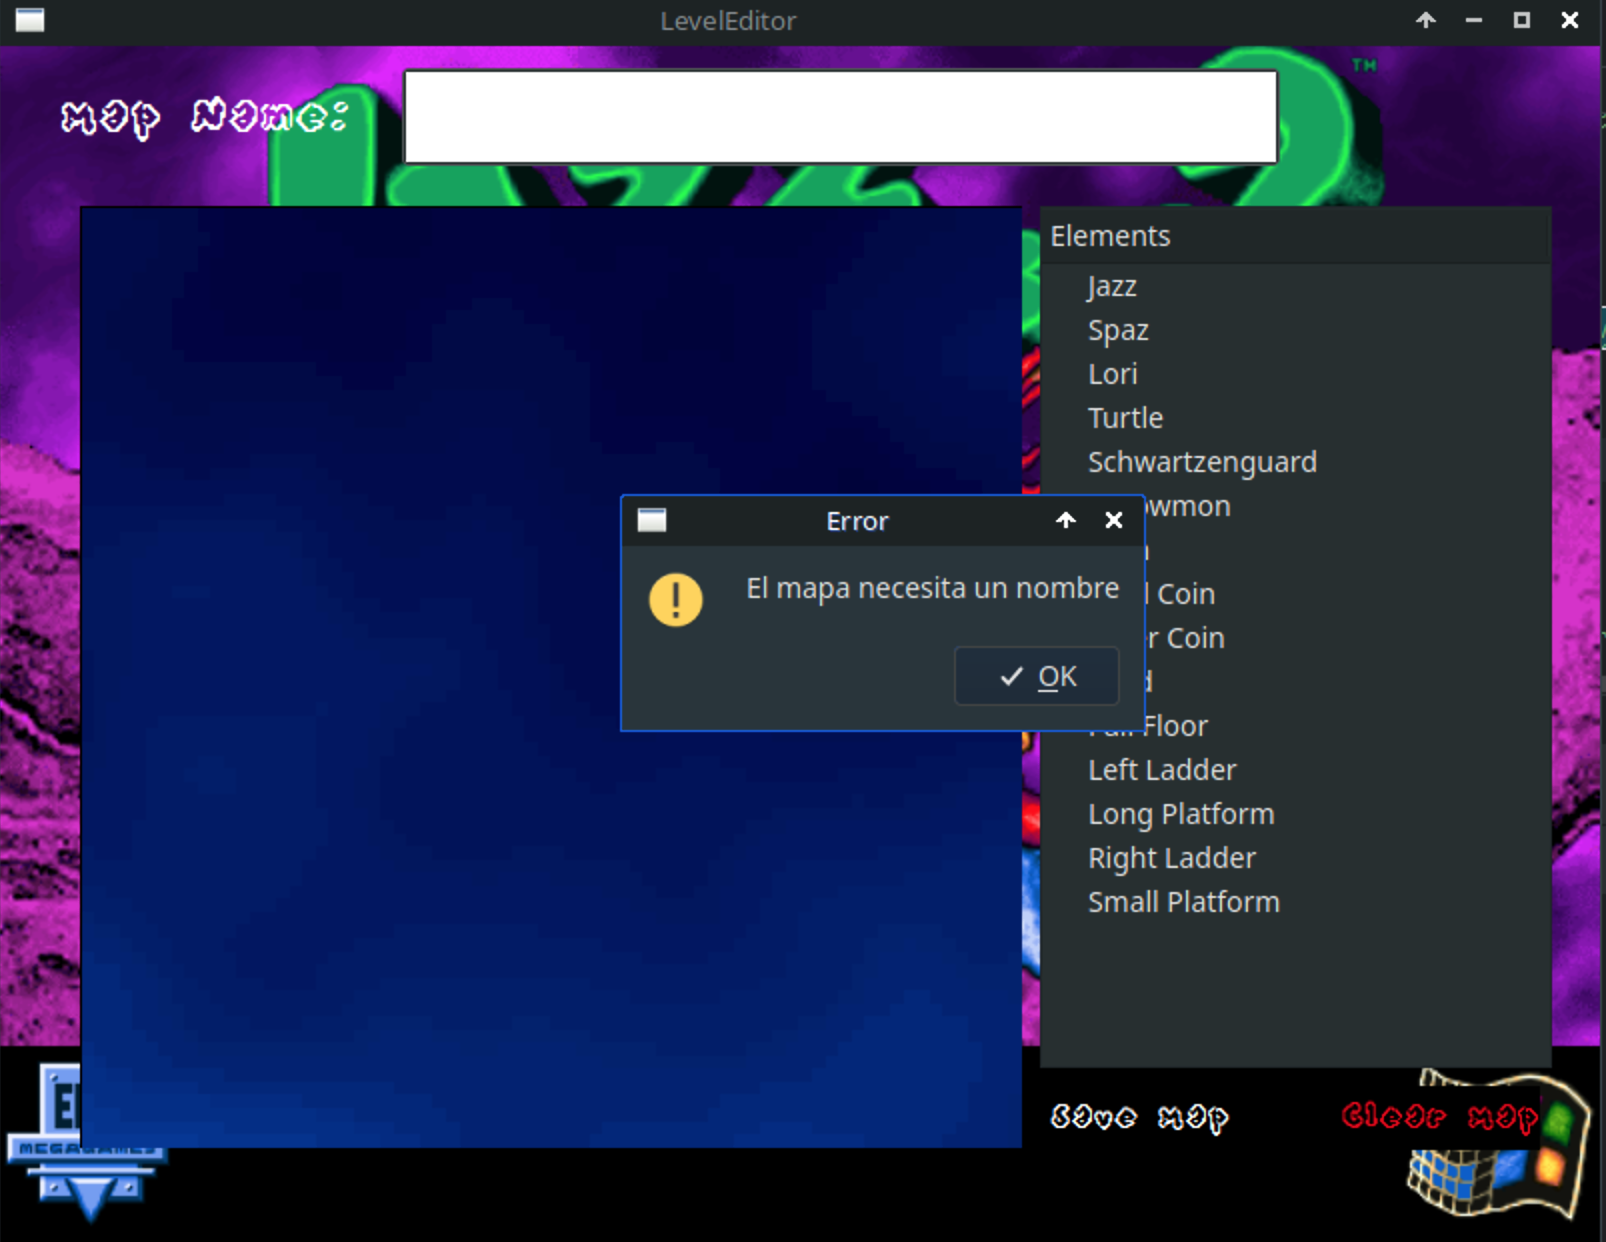
\includegraphics[width=0.8\textwidth]{images/LevelEditor/NoMapName.png}
  \caption{Error en el Editor de Niveles al crear un mapa sin nombre}
  \label{fig:no-map-name}
\end{figure}

Si no tiene elementos:

\begin{figure}[H]
  \centering
  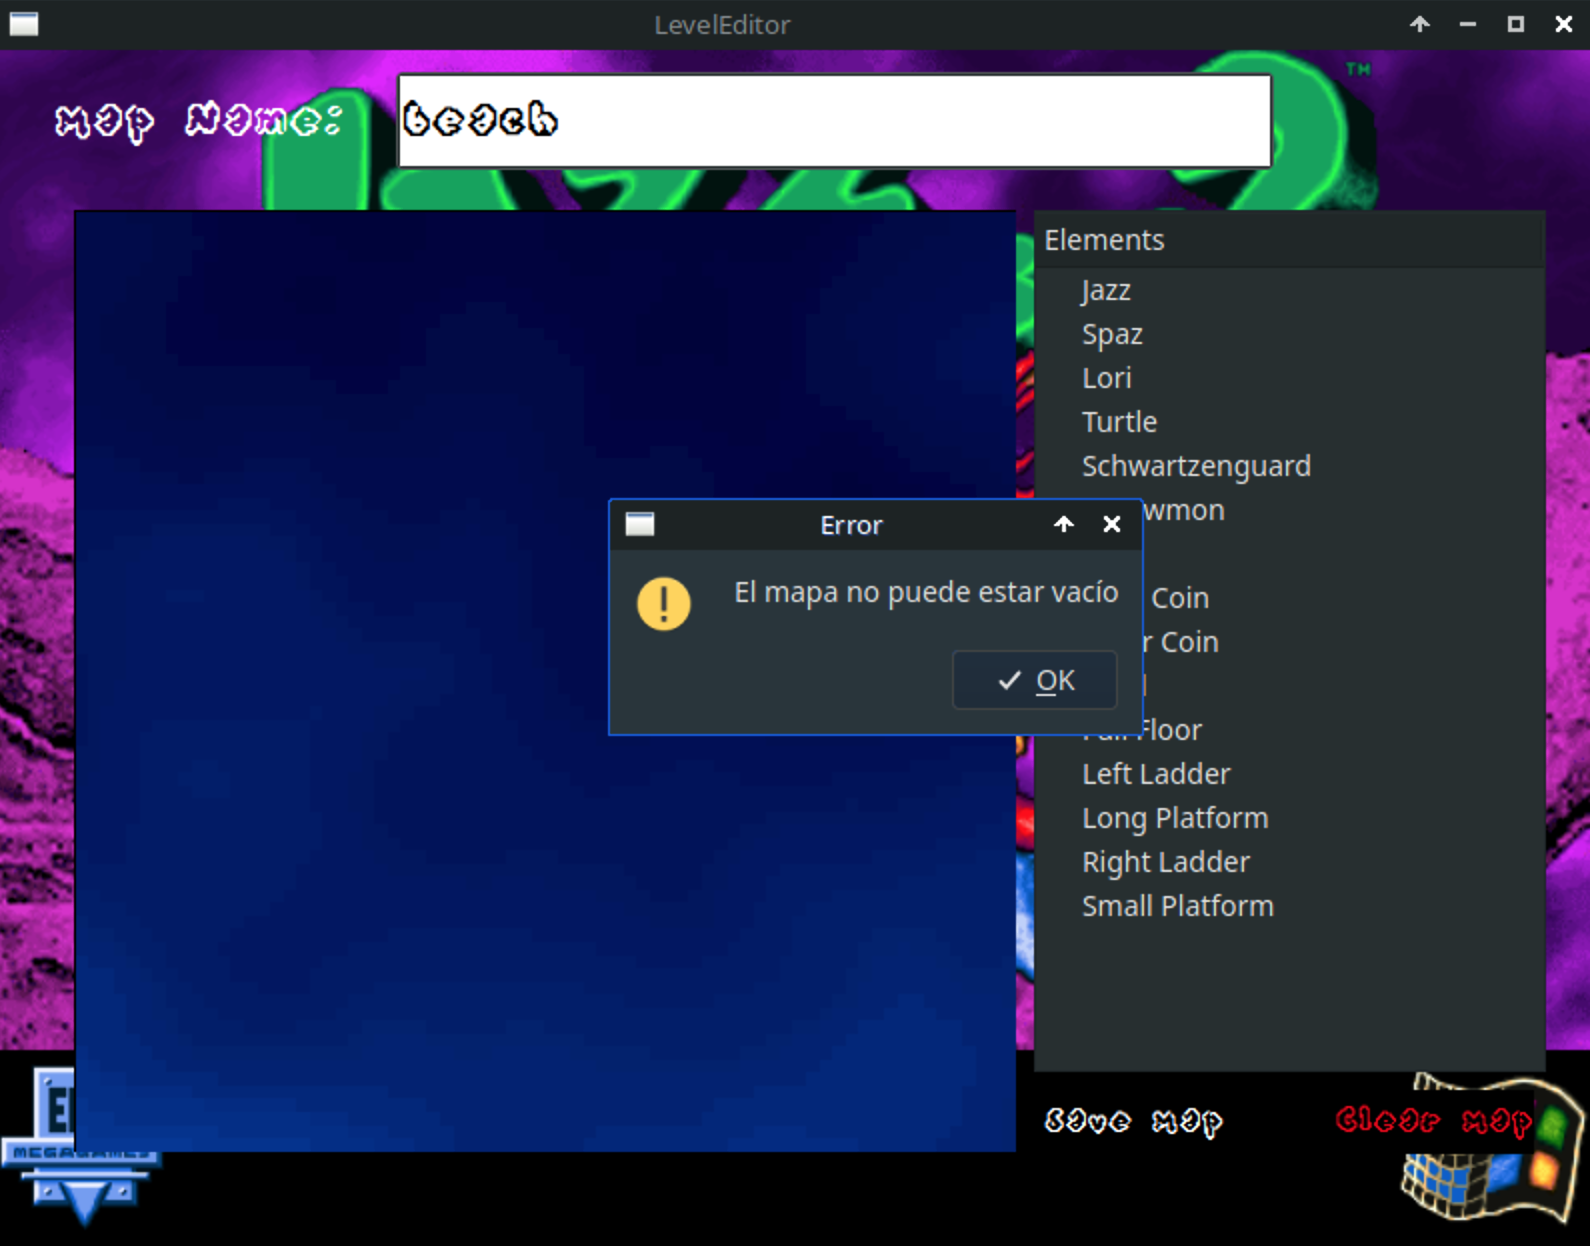
\includegraphics[width=0.8\textwidth]{images/LevelEditor/EmptyMap.png}
  \caption{Error en el Editor de Niveles al crear un mapa sin elementos}
  \label{fig:no-elements}
\end{figure}

Si ya existe un mapa con el mismo nombre:

\begin{figure}[H]
  \centering
  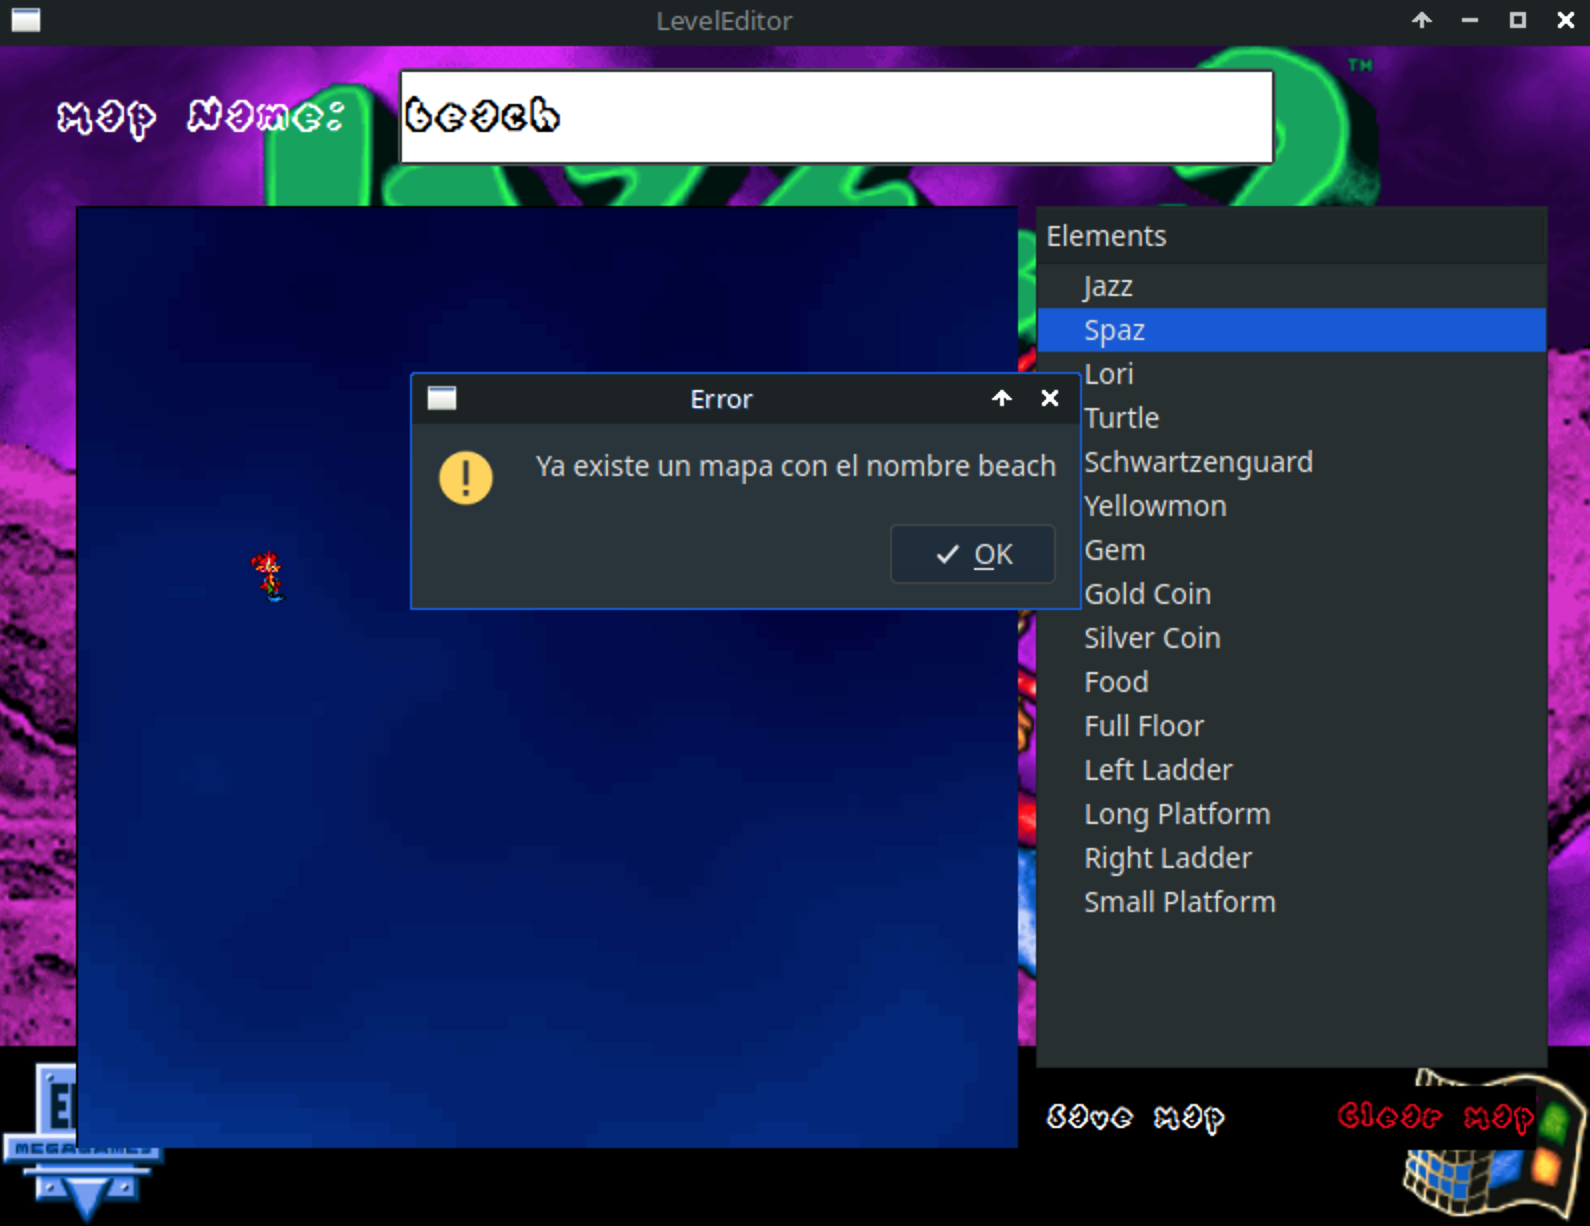
\includegraphics[width=0.8\textwidth]{images/LevelEditor/MapAlreadyExists.png}
  \caption{Error en el Editor de Niveles al crear un mapa con un nombre ya existente}
  \label{fig:map-exists}
\end{figure}

En caso contrario, donde el mapa creado es válido:

\begin{figure}[H]
  \centering
  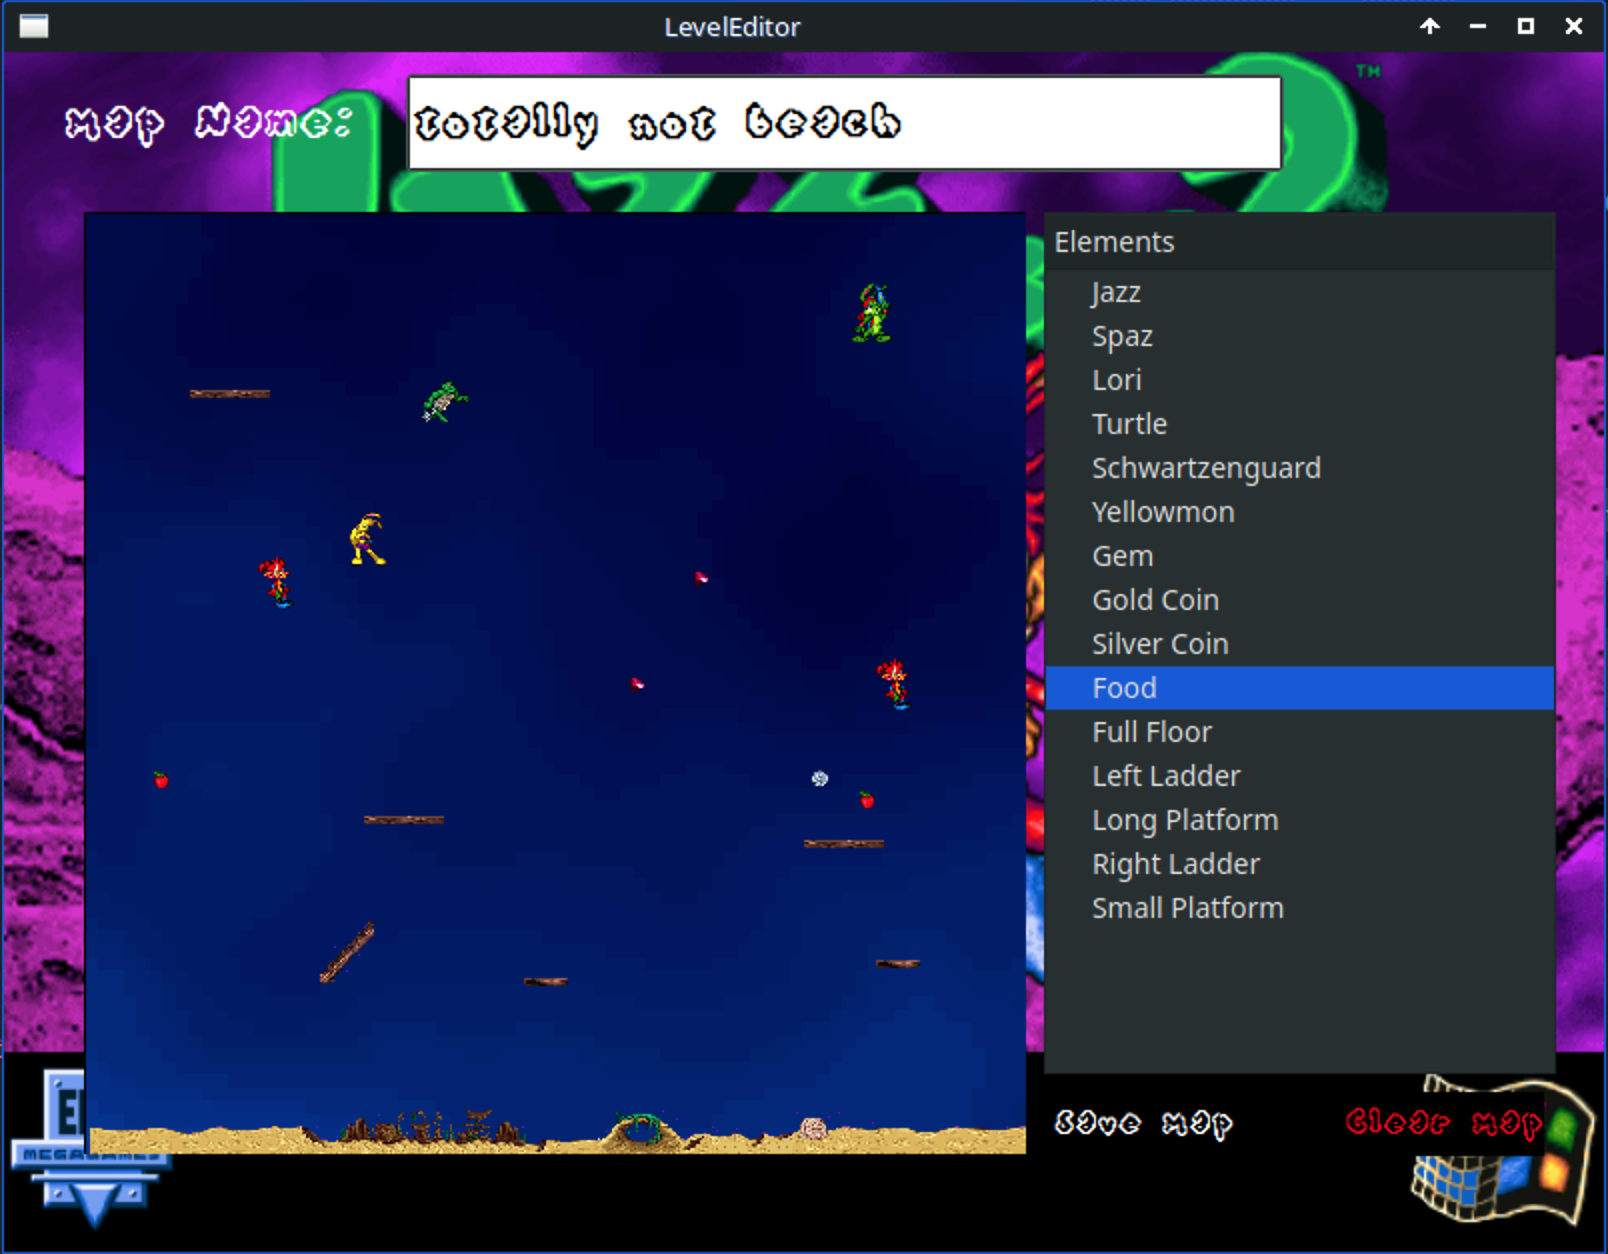
\includegraphics[width=0.8\textwidth]{images/LevelEditor/MapWithElements.png}
  \caption{Mapa válido con elementos}
  \label{fig:valid-map}
\end{figure}

\begin{figure}[H]
  \centering
  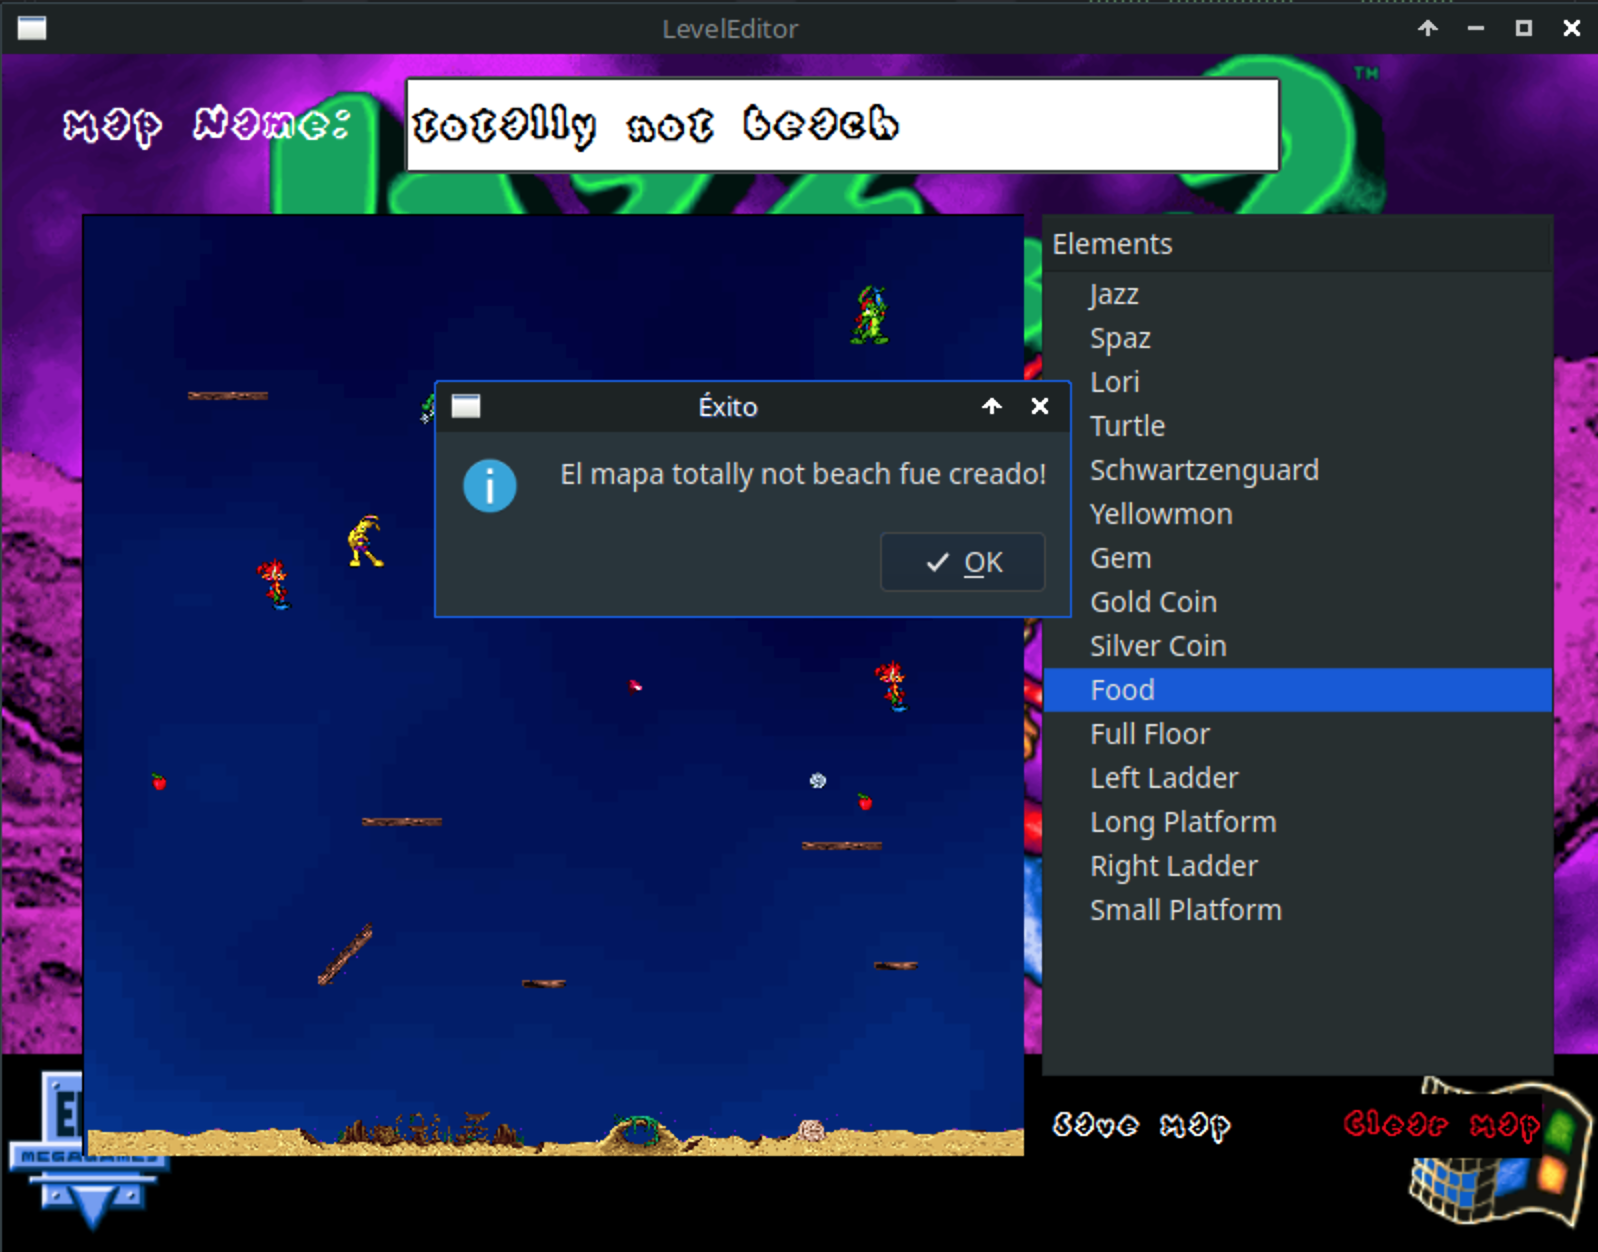
\includegraphics[width=0.8\textwidth]{images/LevelEditor/MapCreated.png}
  \caption{Mapa Creado}
  \label{fig:map-created}
\end{figure}

\end{document}